
%(BEGIN_QUESTION)
% Copyright 2008, Tony R. Kuphaldt, released under the Creative Commons Attribution License (v 1.0)
% This means you may do almost anything with this work of mine, so long as you give me proper credit

The ADC0804 is an example of an integrated circuit analog-to-digital converter (ADC), converting an analog input voltage signal into an 8-bit binary output:

$$\includegraphics[width=15.5cm]{i03270x01.eps}$$

When operated from a 5.0 volt DC power supply in its simplest mode, the ADC0804 converts any DC input voltage between 0.0 volts and 5.0 volts into an 8-bit number at the command of a clock pulse.  A 0.0 volt input yields a binary output (or ``count'') of {\tt 00000000}, of course, while a 5.0 volt input yields a count of {\tt 11111111}.

Complete this table of numbers, relating various DC input voltages with count values (expressed in binary, hex, and decimal) for an ADC0804 having an input range of 0.0 to 5.0 volts DC:

% No blank lines allowed between lines of an \halign structure!
% I use comments (%) instead, so that TeX doesn't choke.

$$\vbox{\offinterlineskip
\halign{\strut
\vrule \quad\hfil # \ \hfil & 
\vrule \quad\hfil # \ \hfil & 
\vrule \quad\hfil # \ \hfil & 
\vrule \quad\hfil # \ \hfil \vrule \cr
\noalign{\hrule}
%
% First row
DC input voltage & Binary count & Hex count & Decimal count \cr
%
\noalign{\hrule}
%
% Another row
0.0 volts & 00000000 &  &  \cr
%
\noalign{\hrule}
%
% Another row
 & 00110011 &  & 51 \cr
%
\noalign{\hrule}
%
% Another row
2.2 volts &  & 70 &  \cr
%
\noalign{\hrule}
%
% Another row
 &  & B3 & 179 \cr
%
\noalign{\hrule}
%
% Another row
 & 11001100 & CC &  \cr
%
\noalign{\hrule}
%
% Another row
5.0 volts & 11111111 &  &  \cr
%
\noalign{\hrule}
} % End of \halign 
}$$ % End of \vbox

\underbar{file i03270}
%(END_QUESTION)





%(BEGIN_ANSWER)

\noindent
{\bf Partial answer:}

% No blank lines allowed between lines of an \halign structure!
% I use comments (%) instead, so that TeX doesn't choke.

$$\vbox{\offinterlineskip
\halign{\strut
\vrule \quad\hfil # \ \hfil & 
\vrule \quad\hfil # \ \hfil & 
\vrule \quad\hfil # \ \hfil & 
\vrule \quad\hfil # \ \hfil \vrule \cr
\noalign{\hrule}
%
% First row
DC input voltage & Binary count & Hex count & Decimal count \cr
%
\noalign{\hrule}
%
% Another row
0.0 volts & 00000000 &  &  \cr
%
\noalign{\hrule}
%
% Another row
1.0 volts & 00110011 & & 51 \cr
%
\noalign{\hrule}
%
% Another row
2.2 volts & 01110000 & 70 & 112 \cr
%
\noalign{\hrule}
%
% Another row
3.51 volts & 10110011 & B3 & 179 \cr
%
\noalign{\hrule}
%
% Another row
4.0 volts & 11001100 & CC & 204 \cr
%
\noalign{\hrule}
%
% Another row
5.0 volts & 11111111 & FF &  \cr
%
\noalign{\hrule}
} % End of \halign 
}$$ % End of \vbox


%(END_ANSWER)





%(BEGIN_NOTES)

The input voltage range of this ADC is 0.0 to 5.0 volts DC, and the output ``count'' range is 0 to 255 (because it outputs an 8-bit unsigned binary number which has this counting range).  Therefore, the relationship between the input voltage and the output count value (in decimal) is a simple proportionality:

$${V_{in} \over 5} = {\hbox{Count} \over 255}$$

Note that all count values are shown rounded {\it down} to the nearest integer value:

% No blank lines allowed between lines of an \halign structure!
% I use comments (%) instead, so that TeX doesn't choke.

$$\vbox{\offinterlineskip
\halign{\strut
\vrule \quad\hfil # \ \hfil & 
\vrule \quad\hfil # \ \hfil & 
\vrule \quad\hfil # \ \hfil & 
\vrule \quad\hfil # \ \hfil \vrule \cr
\noalign{\hrule}
%
% First row
DC input voltage & Binary count & Hex count & Decimal count \cr
%
\noalign{\hrule}
%
% Another row
0.0 volts & 00000000 & 00 & 0 \cr
%
\noalign{\hrule}
%
% Another row
1.0 volts & 00110011 & 33 & 51 \cr
%
\noalign{\hrule}
%
% Another row
2.2 volts & 01110000 & 70 & 112 \cr
%
\noalign{\hrule}
%
% Another row
3.51 volts & 10110011 & B3 & 179 \cr
%
\noalign{\hrule}
%
% Another row
4.0 volts & 11001100 & CC & 204 \cr
%
\noalign{\hrule}
%
% Another row
5.0 volts & 11111111 & FF & 255 \cr
%
\noalign{\hrule}
} % End of \halign 
}$$ % End of \vbox


%INDEX% Electronics review: ADC resolution

%(END_NOTES)


